\documentclass{amsart}
%\usepackage[backend=bibtex8,style=numeric,giveninits=true]{biblatex}
%\addbibresource{formschub.bib}
\usepackage{algorithm}
\usepackage{algpseudocode}
\usepackage{hyperref}
\usepackage{fancyvrb}
\usepackage{amsmath}
\usepackage{amsfonts}
\usepackage{amsthm}
\usepackage{amssymb}
\usepackage{array}
\usepackage{cases}
\usepackage{caption}
\usepackage{xcolor}
\usepackage{tikz}
\usepackage{tikz-cd}
\usepackage{mathtools}
\usetikzlibrary{calc}
\usepackage{centernot}
\usepackage{mathtools}
\usepackage{graphicx}
\usepackage[margin=1in]{geometry}
\usepackage[makeroom]{cancel}
\usepackage{stmaryrd}
\usepackage{stackengine}
\usepackage{mathrsfs}
\usepackage{enumitem}

% Concatenation product on \dcoma: a square cup with a + inside (visually `\sqcupplus`).
\makeatletter
\newcommand{\sqcupplus@inner}[2]{%
  \vcenter{\hbox{\ooalign{%
    \hfil$\m@th#1\sqcup$\hfil\cr
    \hfil\raisebox{0.15ex}{$\m@th#1\scriptscriptstyle+$}\hfil\cr
  }}}%
}
\newcommand{\sqcupplus}{\mathbin{\mathpalette\sqcupplus@inner\relax}}
\makeatother

%\usepackage{unicode-math}
%\usepackage{nicematrix}

%\usepackage{witharrows}

\newtheorem{lemma}{Lemma}[subsection]
\newtheorem{corollary}[lemma]{Corollary}

\newtheorem{proposition}[lemma]{Proposition} 
\newtheorem{proposition2}{Proposition}[section]
\newtheorem{theorem}{Theorem}[section]
\newtheorem{conjecture}[theorem]{Conjecture} 
\newtheorem{observation}{Observation}[section]
\newtheorem{question}{Question}

%\newtheorem{conj}[thm]{Conjecture} 


%%% 
%%% The following gives definition type environments (which only differ
%%% from theorem type invironmants in the choices of fonts).  The
%%% numbering is still tied to the theorem counter.
%%% 

\theoremstyle{definition}
%\newtheorem{definition}{Definition}[section]
%\newtheorem{example}{Example}[section]
\newtheorem{definition}[lemma]{Definition}
\newtheorem{example}[lemma]{Example}
%\newtheorem{algorithm}{Algorithm}
\newtheorem*{note}{Note}
\newtheorem*{method}{Method}
%%
%% Again more of these can be added by uncommenting and editing the
%% following. 
%%

%\newtheorem{note}[thm]{Note}


%%% 
%%% The following gives remark type environments (which only differ
%%% from theorem type invironmants in the choices of fonts).  The
%%% numbering is still tied to the theorem counter.
%%% 


\theoremstyle{remark}

\newtheorem*{remark}{Remark}


%%%
%%% The following, if uncommented, numbers equations within sections.
%%% 

%\numberwithin{equation}{section}
\numberwithin{equation}{subsection}


%%%
%%% The following show how to make definition (also called macros or
%%% abbreviations).  For example to use get a bold face R for use to
%%% name the real numbers the command is $\mathbf{R}.  To save typing we
%%% can abbreviate as

\newcommand{\R}{\mathbf{R}}  % The real numbers.

%%
%% The comment after the definition is not required, but if you are
%% working with someone they will likely thank you for explaining your
%% definition.  
%%
%% Now add you own definitions:
%%

%%%
%%% Mathematical operators (things like sin and cos which are used as
%%% functions and have slightly different spacing when typeset than
%%% variables are defined as follows:
%%%

\DeclareMathOperator{\sch}{\mathfrak{S}}
\newcommand{\shup}{{\uparrow}}
\newcommand{\downvar}[1]{\stackrel{#1}{\searrow}}
\newcommand{\wof}[1]{w_{#1}}
\newcommand{\rcdd}{\mathfrak{d}}
\newcommand{\wtt}{\mathtt{wt}}
\newcommand{\QY}{\ensuremath{\mathbb{QY}}}
\newcommand{\tom}[1]{\xrightarrow{#1}}
\newcommand{\Tom}[1]{\xRightarrow{#1}}
\newcommand{\mot}[1]{\xleftarrow{#1}}
\newcommand{\grass}{\mathcal{G}}
\newcommand{\plac}{\mathrm{Plac}}

\newcommand{\cperm}[1]{\llbracket #1\rrbracket}
\newcommand{\cpcf}[5]{d^{#1,#2}_{#3}\left(#4\mid #5\right)}
% simplified product notation
\newcommand{\smpfu}{\mathsf{\Pi}}
\newcommand{\smpr}[3]{\ensuremath{}\smpfu\left( #1 \mid #2_{[#3]}\right)}
%\newcommand{\smpre}[2]{\ensuremath{}\smpfu\left( #1 \mid #2\right)}
\newcommand{\smpre}[2]{\ensuremath{}\prod_{b\in #2}(#1-b)}
\newcommand{\qr}{\mathfrak{R}}
\newcommand{\rtt}{\mathtt{rt}}
\newcommand{\trm}{\mathtt{trim}}
\newcommand{\zeromap}{\mathcal{Z}}
\newcommand{\hr}{\mathtt{ht}}
\newcommand{\clp}{\mathtt{clip}}
\newcommand{\BRC}{\mathcal{BRC}}
\newcommand{\RC}{\mathcal{RC}}
\newcommand{\lzeromap}{\mathscr{Z}}
\newcommand{\lmap}{\mathscr{L}}
\newcommand{\ltb}{\mathrm{little}}
\newcommand{\slide}{\mathfrak{F}}
\newcommand{\ttrim}{\mathfrak{T}}
%\newcommand{\shifthom}{\operatornamewithlimits{\raisebox{1ex}{$\stackrel{\blacktriangleright}{\mathbf{\_}}$}}\limits}

%\newcommand{\shifthom}{\operatornamewithlimits{\raisebox{1ex}{$\blacktriangleright$}}\limits}

\newcommand{\shifthom}{\operatornamewithlimits{\triangleright}\limits}


%\newcommand{\shiftvby}[1]{\ensuremath{\resizebox{\width}{\heightoff}{$\shifthom_{#1}$}}}

\newcommand{\shiftvby}[1]{\shifthom_{#1}}

\newcommand*\circled[1]{%
	\tikz[baseline=(char.base)]{
		\node[shape=circle,draw,inner sep=0.1pt] (char) {#1};
	}%
}
\newcommand\mycircled[1]{\makebox[0pt]{\circled{#1}}}
\newcommand{\tb}{\textbullet}
\newcommand{\xr}[1]{\ensuremath{{}\xrightarrow{[#1]}{}}}
\newcommand{\rd}[1]{\ensuremath{\mathcolor{red}{\mathbf{#1}}}}
\newcommand{\mc}[1]{\ensuremath{\mycircled{#1}}}
\newcommand{\desc}{\mathrm{Desc}}%
\newcommand{\SSYT}{\mathrm{SSYT}}
%\newcommand{\schv}[2]{\operatornamewithlimits{\sch_{\mathit{#2}}}\limits_{\negphantom{{}_{\mathit{#2}}}\negvphantom{{}_{\mathit{#2}}}#1}}

%\newcommand{\schv}[2]{\setstackgap{S}{0pt}\setstackgap{L}{0pt}\stackMath\stackunder{\sch_{#2}}{\negphantom{\scriptstyle{#2}}\!{\scriptscriptstyle{#1}}}}

\newcommand{\schv}[2]{\shiftvby{#1}\!\sch_{#2}}

%\newcommand{\shiftvby}[1]{\makebox[0pt]{$\triangleright$}#1}



%\newglossary[slg]{symbolslist}{syi}{syg}{List of symbols}
%\makeglossaries

%\begin{itemize}
%	\item Elements of $S_\infty$ $c{[}p,q{]}$, $d{[}p,q{]}$, $r{[}p,q{]}$, homomorphism $\sigma_p:S_\infty\to S_\infty$: Definition \ref{definition:specelem}	

%	\item  Relations between elements of $S\infty$ $\tom{k},\Tom{k}$: Definition \ref{definition:pierisymb}

%	\item Code, dual code, $\code(w)$, $\code^*(w)$, dominant permutations, the dominant approximation $\dom(v)$: Definition \ref{definition:codestuff}

%	\item Function/sets of permutations related to pulling out variables from Schubert polynomials $\varphi_{i,n}$, $\mathcal{D}_i(v)$, $Q_i(v',v)$: Definition \ref{definition:polysequence}

%	\item Flattening function $\phi_i:S_\infty\to S_\infty$, domination relation between permutations: Definition \ref{definition:domination}

%	\item Special polynomials $H_p(x;y)$, $E_p(x;y)$, $\smpr{x_1}{y}{p}$: Definition \ref{definition:hp}

%	\item Polynomial variable omission $x^{(i)}$, subscript substitution $y_A$, index shift function $\shiftvby{i}$: Definition \ref{definition:pv}
%\end{itemize}

\newcommand{\dsch}{\ensuremath{\Xi}}
\newcommand{\coma}{\mathcal{A}}
\newcommand{\dcoma}{\mathcal{D}}



%%
%% This is the end of the preamble.
%% 
\title{A Littlewood--Richardson rule for forest polynomials via operations on RC graphs}
\author{Matthew J. Samuel}

%\newcommand{\tomm}[2]{\xrightarrow{#1}_{#2}}
%\counterwithout{equation}{section}
%\setcounter{section}{-1}
\newcommand{\shuff}[2]{\mathcal{S}\mathcal{H}_{#1}^{#2}}
\newcommand{\dom}{\mathfrak{d}}
\newcommand{\ldom}{\dom^*}
\newcommand{\code}{\mathfrak{c}}
\newcommand{\ducode}{\overline{\mathfrak{c}}}
\newcommand{\forest}{\mathfrak{P}}
\newcommand{\fcode}{\mathfrak{c}_\forest}
\newcommand{\finv}{P_{\forest}}

\newcommand{\maxd}{\mathfrak{m}}
%\newcommand{\ddv}[1]{{{}_{{\scriptscriptstyle (#1)}}\partial}}
\newcommand{\ddv}[1]{\delta}
%\newglossary[slg]{symbolslist}{syi}{syg}{Symbolslist}
%\GlsXtrLoadResources
%[src={symbols},sort=use,type=main,
%	group=specelem]
%\glsaddstoragekey{group}{}{\grouplabel}
%\glsxtrsetgrouptitle{specelem}{}
\newcommand{\xleadsto}[2][]{\overset{#2}{\leadsto}}

\newcommand{\ins}[2]{{#2\xleadsto{#1}}}





%\newglossary[slg]{symbol}{sot}{stn}{Symbols}
%\makeglossaries

\begin{document}

\begin{abstract}
\end{abstract}

	\maketitle


\section{Introduction}


% \section{Set-valued inversions tableaux}
% \begin{definition}

% Let $w$ be a permutation such that $\maxd(w)\leq n$. Suppose $T:I(w)\to \mathbf{2}^{[n]}\setminus \{\varnothing\}$ is a function mapping a root to a nonempty subset of $[n]$. Define relations $\leq$ and $<$ on these sets by declaring that $A\leq B$ if $\max(A)\leq \min(B)$ and $A<B$ if $\max(A)<\min(B)$. 
% We say that $T$ is a \emph{set-valued inversions tableau} if the following conditions are satisfied:
% \begin{itemize}
%   \item If $i < j < k$ and $(i,j),(j,k),(i,k)\in I(w)$, then either $T(i,j) \leq T(i,k) \leq T(j,k)$ or $T(j,k) \leq T(i,k) \leq T(i,j)$.
%   \item If $i>0$ and $j<k$ are such that $(i,j),(i,k)\in I(w)$, then $T(i,j) < T(i,k)$.
%   \item $T(i,i+1)\leq \{i\}$ for all $i$.

% \end{itemize}
% For $(i,j)\in I(w)$, define $\lambda_T(i,j)$ as follows. Suppose $T(i,j) = r$. Let $(i,k)$ be the root such that $T(i,k)=r$ and $k$ is minimal. Then $\lambda_T(i,j) = i + j + 1 - k$.
% \end{definition}

% \begin{theorem}
% Suppose $w$ is a permutation. Then we have the following formula for the double Grothendieck polynomial of $w$:
% $$\mathfrak{G}_w^{(\beta)}(x;y) = \sum_{T} \prod_{(i,j)\in I(w)} \beta^{|T(i,j)| - 1} \prod_{r\in T(i,j)} x_r \oplus y_{\lambda_T(i,j) - r}$$
% where the sum is over all set-valued inversions tableaux of $w$. 
% \end{theorem}

% \begin{definition}
% An \emph{staircase word graph} is simply a subset of $\mathbb{N}^2$. We impose the same ordering on these as RC graphs. That is, we say that $(a,b)\leq (c,d)$ if $a<c$ or $a=c$ and $b > d$. We define $\mathbf{word}(G)$ to be the word obtained by reading the elements $i + j - 1$ in the linear order given by $\leq$. We then say that $\wof{G}$ is the Demazure product of $\mathbf{word}(G)$.

% For a set-valued inversions tableau $T$, we can define a staircase word graph $G$ as follows. If $w$ is the identity, then $G$ is the empty set. Otherwise, let $n$ be the maximum value that is contained in $T(i,j)$ for some $(i,j)\in I(w)$. Choose $i$ and $j$ such that $T(i,j)=n$ and $i + j$ is as small as possible. Necessarily, $j=i+1$, or in other words $i$ is a right descent of $w$. If $|T(i,i+1)| > 1$, remove $n$ from $T(i,i+1)$ to obtain a new function $T':I(w)\to \mathbf{2}^{[n]}\setminus \{\varnothing\}$. If $|T(i,i+1)|=1$, then let $T':I(ws_i)\to \mathbf{2}^{[n]}\setminus \{\varnothing\}$ be the function defined by
% $$T'(a,b) = T(s_i(a),s_i(b))$$
% for all $(a,b)\in I(ws_i)$.

% It is straightforward to check that $T'$ is a set-valued inversions tableau, either for $w$ if $|T(i,i+1)| > 1$ or for $ws_n$ if $|T(i,i+1)| = 1$. Let $G'=\Phi(T')$. Then let $\Phi(T)=G'\cup \{(n,i+1-n)\}$. 
% \end{definition}

% \begin{proposition}
% $\Phi$ is a bijection between set-valued inversions tableaux of $w$ with maximum value $n$ and staircase word graphs $G$ such that $\wof{G} = w$ and $a\leq n$ for all $(a,b)\in G$.
% \end{proposition}
% \begin{proof}
%   If $|T(i,j)|=1$ for all $(i,j)\in I(w)$, then $T$ is just an ordinary inversion tableau and $\Phi(T)$ is just the usual RC graph associated to $T$. In this case, the result is \cite{axelrodfreed2025inversionstableaux}. Otherwise, we prove this by induction on the maximum size of $|T(i,j)|$. Suppose this maximum size is $m>1$ and we have proved the result for all set-valued inversions tableaux with maximum size less than $m$. We may assume without loss of generality that $m$ is the maximum value that is contained in $T(i,j)$ for some $(i,j)\in I(w)$ by removing elements below. In that case, $m\in T(i,i+1)$ for some $i$. Let $T'$ be the set-valued inversions tableau obtained by removing $m$ from $T(i,i+1)$ if $|T(i,i+1)| > 1$ or by applying the transformation described in the definition of $\Phi$ if $|T(i,i+1)|=1$. By the inductive hypothesis, $\Phi(T')$ is a staircase word graph such that $\wof{\Phi(T')} = w$ or $\wof{\Phi(T')} = ws_i$ and $a\leq n$ for all $(a,b)\in \Phi(T')$. In either case, we have $\wof{\Phi(T)} = w$. It is also clear that $a\leq n$ for all $(a,b)\in \Phi(T)$. This proves that $\Phi(T)$ is a staircase word graph with the desired properties.

%   Let $G$ be a staircase word graph. Define $\Psi(G)$ to be empty if $G$ is empty. Otherwise, let $(i,j)$ be the maximum element of $G$ and let $G' = G\setminus \{(i,j)\}$. Let $w'=\wof{G'}$. Let $d=i + j - 1$. If $\ell(w's_d) > \ell(w')$, then let
% $$\Psi(G)(a,b) = \begin{cases}
% \Psi(G')(s_d(a),s_d(b)) & \text{if } (a,b)\in I(w)\setminus\{(i,j)\}\\
% \{d\} & \text{if } (a,b) = (i,j)
% \end{cases}$$
% If $\ell(w's_d) < \ell(w')$, then let
% $$\Psi(G)(a,b) = \begin{cases}
% \Psi(G')(a,b) & \text{if } (a,b)\in I(w)\setminus\{(i,j)\}\\
% \Psi(G')(a,b)\cup \{d\} & \text{if } (a,b) = (i,j)
% \end{cases}$$
% \end{proof}

% \begin{definition}
% Define the isobaric divided difference operator
% $$\pi^i = \partial^i(1+\beta x_{i+1})$$
% Note the Leibniz formula
% $$\pi^i(fg) = (\pi^i+\beta s_i)(f)g + f\pi^i(g)$$
% \end{definition}

\section{Nil-Coxeter action}

Let $R$ be an RC graph and let $i>0$ be an integer. We define $\rcdd^iR$, an element of $\RC$, as follows. Define
$$\rcdd^iR=0$$
unless $s_i$ is a right descent of $\wof{R}$ and there exists $(i,j)\in R$ such that $\rtt_R(i, j) = (i, i+1)$. If these latter two conditions are satisfied, define 
$$R'=R\setminus \{(i, j)\}$$
where $\rtt_R(i,j) = (i, i+1)$. If $e_i(R')\neq \emptyset$, define $\rcdd^iR=0$. Otherwise, define
$$\rcdd^iR = \sum_{p=0}^{\varphi_i(R')}f_i^pR'$$
\begin{lemma} \label{lemma:divdiffunique}
	Let $R$ be an RC graph and let $i>0$ be an integer. If $s_i$ is not a right descent of $\wof{R}$, then there is a unique $R'$ such that the coefficient of $R$ in $\rcdd^iR'$ is $1$, and for other $R'$ the coefficient is $0$.
\end{lemma}
\begin{proof}
	Suppose $s_i$ is not a right descent of $\wof{R}$. Assume without loss of generality that $e_iR = \emptyset$. If $(i+1, 1)\notin R$, then $(i,1)\notin R$ because $s_i$ is not a right descent of $\wof{R}$. In that case, let $R' = R\cup\{(i,1)\}$. Then 
	$$\rcdd^iR' = R + \text{other terms}$$ 
	If instead $(i+1, 1)\in R$, since $e_i(R)=\emptyset$ it follows that $(i, 1)\in R$, and if $j$ is the maximum value such that $(i+1,j')\in R$ for all $j'<j$, it follows that $(i,j')\in R$ for all $j'<j$. We must have that $(i,j+1)\notin R$, because $\rtt_R(i, j+1)=(i, i+1)$. Setting $R'=R\cup \{(i, j+1)\}$ gives us the result.
\end{proof}

\begin{theorem} \label{theorem:divdiffschubert}
	Suppose $w\in S_\infty$ and $i >0$. If $i$ is not a right descent of $w$, then
	$$\rcdd^i\mathcal{S}_w(n) = 0$$
	Otherwise,
	$$\rcdd^i\mathcal{S}_w(n) = \mathcal{S}_{ws_i}(n)$$
\end{theorem}
\begin{proof}
	The result is trivial if $i$ is not a right descent of $w$. Suppose $i$ is a right descent of $w$. By Lemma \ref{lemma:divdiffunique}, for each RC graph $R$ such that $\wof{R} = ws_i$, there is a unique RC graph $R'$ such that the coefficient of $R$ in $\rcdd^iR'$ is $1$. Since $\wof{R'} = w$, the result follows.
\end{proof}

\begin{corollary} \label{corollary:generateschubert}
Suppose $R$ is an RC graph such that $\wof{R} = w$ is dominant. Then for any reduced word $(s_{i_1}, s_{i_2}, \ldots, s_{i_m})$ for a permutation $u$ such that
$$\ell(wu^{-1}) = \ell(w) - \ell(u)$$
we have that
$$\rcdd^{i_1}\rcdd^{i_2}\cdots \rcdd^{i_m}R = \mathcal{S}_{wu^{-1}}(n)$$
for sufficiently large $n$.
\end{corollary}


\begin{definition}
For a permutation $w$, define the \emph{principal RC graph} $R^0(w)$ of $w$ to be
$$R^0(w) = \{(i,j)\mid 1\leq j\leq \code_i(w)\}$$

We say that row $i$ of an RC graph $R$ has a \emph{ledge} at column $j$ if the configuration of boxes in rows $i$ and $i+1$ satisfy $(i,j)\in R$, $(i+1,j)\notin  R$, $\rtt_R(i,j)=(i,i+1)$, and for all $j' < j$ we have that $(i,j')\in R$ and $(i+1,j')\in R$, as shown in in Figure \ref{figure:ledge}.
\end{definition}

\begin{proposition} \label{proposition:divdiffprincipal}
Let $R$ be an RC graph and let $w=\wof{R}$. Then the following are equivalent.
\begin{enumerate}
\item for any reduced word $(s_{i_1}, s_{i_2}, \ldots, s_{i_m})$ for $w$, we have
$$\rcdd^{i_1}\rcdd^{i_2}\cdots \rcdd^{i_m}R \neq 0$$

\item $R = R^0(w)$.
\end{enumerate}
\end{proposition}
\begin{proof}
For (1)$\Rightarrow$(2), we proceed by induction on length. For (1) to be true, in particular if $n=\maxd(\wof{R})$ we have that $(n,1)\in R$. Applying $\rcdd^n$ and lowering operators (necessarily maximally) results in a term being an RC graph which has the same recursive property, which by the inductive hypothesis is $R^0(ws_n)$, which implies that row $n$ of $R$ has length $\code_n(w)$. Choosing our reduced word carefully, we obtain in the process as some nonzero term an RC graph for $w'$ with $\code_k(w') = \code_k(w)$ for all $k<n$ and $\code_n(w')=0$ that has the same property, and hence is principal by the induction hypothesis. It follows that $R$ is principal as well.

For (2)$\Rightarrow$(1), we again proceed by induction on length. If $w$ has no descents, the statement is vacuous. For a principal RC graph $R^0(w)$ for some $w$ with $\ell(w)>0$ and we have the result for smaller lengths, suppose $i$ is a descent of $w$. Then $\code_i(w) > \code_{i+1}(w)$. In particular, if we let $j = \code_{i+1}(w) + 1$, then $(i,j)$ is a ledge of $R^0(w)$. Applying $\rcdd^iR^0(w)$, the lowest weight in the sum is in fact $R^0(ws_i)$. It follows by induction that applying the sequence of divided difference operators corresponding to a reduced word for $w$ to $R^0(w)$ yields the empty RC graph with a coefficient of $1$.
\end{proof}

  \begin{definition}
We say that row $i$ of an RC graph $R$ has a \emph{ledge} at column $j$ if the configuration of boxes in rows $i$ and $i+1$ satisfy $(i,j)\in R$, $(i+1,j)\notin  R$, $\rtt_R(i,j)=(i,i+1)$, and for all $j' < j$ we have that $(i,j')\in R$ and $(i+1,j')\in R$, as shown in Figure \ref{figure:ledge}.
\end{definition}

\begin{lemma} \label{lemma:block_structure}
Suppose $\rcdd^iR\neq 0$. Then the following hold:
\begin{enumerate}
\item \label{item:e_i_empty} $e_iR=\emptyset$.
\item \label{item:blocky} There exists a $j\geq 1$ such that $R$ has a ledge at column $j$.
\end{enumerate}
\end{lemma}
\begin{proof}
If $\rcdd^iR\neq 0$, this means that the root $(i, i+1)$ is in row $i$. This happens precisely when we have an element $(i,j)\in R$ such that $(i+1, j)\notin R$, but $(i, j')\in R$ and $(i+1, j')\in R$ for all $1\leq j'<j$. It follows that if $e_iR\neq \emptyset$, then $e_i(R\setminus\{(i,j)\})\neq \emptyset$. This means that $\rcdd^iR=0$, which contradicts the assumption and proves (\ref{item:e_i_empty}).

For (\ref{item:blocky}), by assumption we knnow that there exists some $(i,j)\in R$ with $\rtt_R(i,j)=(i,i+1)$. Recall that $\rtt_R(i,j) = (\wof{R[i,j]}^{-1}(i + j -1), \wof{R[i,j]}^{-1}(i+j))$. Reasoning directly shows that in order for the first component to be $i$, the graph must satisfy the condition that for all $j' < j$ we have that $(i,j')\in R$. Furthermore, in order to satisfy the condition that $R[i,j]^{-1}(i+j) = i+1$, we cannot have that $(i+1,j)\in R$, and this also imposes the requirement that for all $j' < j$ we have that $(i+1,j')\in R$.
\end{proof}




\begin{figure}[h]
\centering
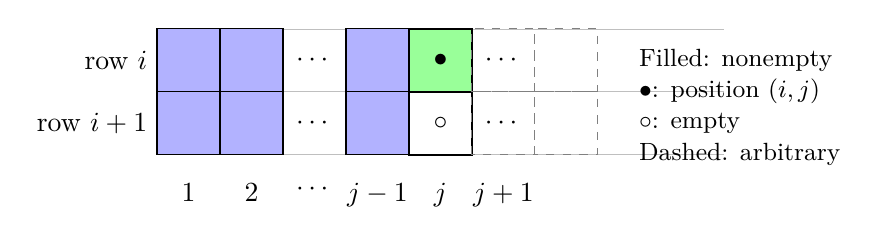
\begin{tikzpicture}[scale=0.8]
  % Draw grid
  \draw[lightgray, very thin] (0,0) -- (9,0);
  \draw[lightgray, very thin] (0,1) -- (9,1);
  \draw[lightgray, very thin] (0,2) -- (9,2);
  
  % Row i boxes - columns 1 and 2
  \foreach \x in {0,1} {
    \fill[blue!30] (\x,1) rectangle (\x+1,2);
    \draw (\x,1) rectangle (\x+1,2);
  }
  
  % Row i+1 boxes - columns 1 and 2
  \foreach \x in {0,1} {
    \fill[blue!30] (\x,0) rectangle (\x+1,1);
    \draw (\x,0) rectangle (\x+1,1);
  }
  
  % Ellipses between 2 and j-1
  \node at (2.5,1.5) {$\cdots$};
  \node at (2.5,0.5) {$\cdots$};
  
  % Column j-1
  \fill[blue!30] (3,1) rectangle (4,2);
  \draw (3,1) rectangle (4,2);
  \fill[blue!30] (3,0) rectangle (4,1);
  \draw (3,0) rectangle (4,1);
  
  % Position (i,j) - nonempty
  \fill[green!40] (4,1) rectangle (5,2);
  \draw[thick] (4,1) rectangle (5,2);
  \node at (4.5,1.5) {$\bullet$};
  
  % Position (i+1,j) - empty (white)
  \fill[white] (4,0) rectangle (5,1);
  \draw[thick] (4,0) rectangle (5,1);
  \node at (4.5,0.5) {$\circ$};
  
  % Visual ellipses for "anything can happen" to the right
  \draw[dashed, gray] (5,1) rectangle (6,2);
  \node at (5.5,1.5) {$\cdots$};
  \draw[dashed, gray] (5,0) rectangle (6,1);
  \node at (5.5,0.5) {$\cdots$};
  
  \draw[dashed, gray] (6,1) rectangle (7,2);
  \draw[dashed, gray] (6,0) rectangle (7,1);
  
  % Labels
  \node[left] at (0,1.5) {row $i$};
  \node[left] at (0,0.5) {row $i+1$};
  
  % Column labels
  \node[below] at (0.5,-0.3) {$1$};
  \node[below] at (1.5,-0.3) {$2$};
  \node[below] at (2.5,-0.3) {$\cdots$};
  \node[below] at (3.5,-0.3) {$j-1$};
  \node[below] at (4.5,-0.3) {$j$};
  \node[below] at (5.5,-0.3) {$j+1$};
  
  % Legend
  \node[anchor=west, align=left] at (7.5,1.5) {\small Filled: nonempty};
  \node[anchor=west, align=left] at (7.5,1) {\small $\bullet$: position $(i,j)$};
  \node[anchor=west, align=left] at (7.5,0.5) {\small $\circ$: empty};
  \node[anchor=west, align=left] at (7.5,0) {\small Dashed: arbitrary};
\end{tikzpicture}
\caption{Configuration for rows $i$ and $i+1$ for a ledge at $(i,j)$.}
\label{figure:ledge}
\end{figure}




\begin{theorem}
The crystal divided difference operators satisfy the relations:
$$\rcdd^i\rcdd^i = 0$$
$$\rcdd^i\rcdd^j = \rcdd^j\rcdd^i\quad\mbox{for }|i-j|>1$$
$$\rcdd^i\rcdd^{i+1}\rcdd^i = \rcdd^{i+1}\rcdd^i\rcdd^{i+1}$$
\end{theorem}

\begin{proof}
The first and second relations are not difficult. Otherwise, assume without loss of generality that $i=1$. For an RC graph with precisely three rows, let us consider applying $\rcdd^1\rcdd^2\rcdd^1$. Suppose $\code(w) = (a, b, c)$. It is well known that if $m=\min(a, b, c)$, then the first $m$ columns of $R$ are completely full, hence without loss of generality let us assume that $m=0$. The only way the braid relation can apply to yield a nonzero result, therefore, is if $a>b>c=0$. Since this yields a dominant permutation, it follows that $R$ is the unique RC graph for $w$. Applying the braid relation in either direction yields the complete sum of RC graphs for the permutation with code $(0, a - 1, b - 2)$ by application of Corollary \ref{corollary:generateschubert}. By transfer, this result also applies to the last two or three rows of any RC graph with respect to the code.

Considering a general RC graph, we may similarly assume that $\code_3(w)=0$ by removing full columns, since only ledges will yield nonzero results. If there are extra elements in the first three rows that are not in the implied dominant block, then they all satisfy $r + c - 1 > \code_r(w) + 1$, where $r\in \{1,2,3\}$ and the extra element is at row $(r,c)$, since they have come down from a row past row $4$ (with respect to the principal RC graph). Elements with $r + c - 1 > \code_1(w) + 1$ can be seen to have no essential interaction with rows $1$, $2$, and $3$ and can be disregarded. We are left with the configuration in Figure \ref{figure:whatsleft}.

In this situation, without ambiguity, application of the braid triple in either direction will delete the immobile $(2,1)$, $(1, \code_2(w) + 1)$, and $(1,1)$. Without application of any lowering operators, simply deleting these elements yields the highest weight of the crystal component containing $R$ with respect to the first three rows. Since we may apply $\clp^3(R)$ to obtain a Demazure crystal, the lowering operators transitively generate the sum. To see that we indeed get all of them, we note that for this highest weight $R' = \clp^3(R)$, application of $\rcdd^1\rcdd^2\rcdd^1$ should yield elements of the form
$$f_1^{a_1}f_2^{a_2}f_1^{a_3}R'$$
and for the other direction,
$$f_2^{b_1}f_1^{b_2}f_2^{b_3}R'$$
These are two distinct parametrizations of the Demazure crystal $B_{s_1s_2s_1}(\lambda)=B_{s_2s_1s_2}(\lambda)$ with highest weight $\lambda$, yielding the same elements.
\end{proof}


\newcommand{\BRF}{\mathcal{BRF}}
\newcommand{\RF}{\mathcal{RF}}
\newcommand{\cs}{\widetilde{s}}


\begin{figure}[h]
\centering
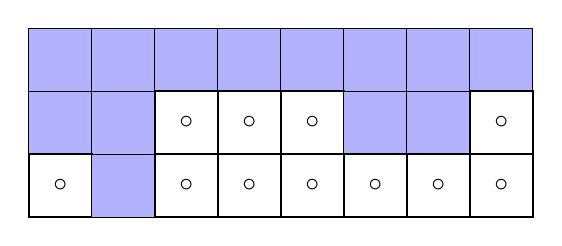
\begin{tikzpicture}[scale=0.8]
  % Row 1 (top row) - fully filled
  \fill[blue!30] (0,2) rectangle (1,3);
  \draw (0,2) rectangle (1,3);
  \fill[blue!30] (1,2) rectangle (2,3);
  \draw (1,2) rectangle (2,3);
  \fill[blue!30] (2,2) rectangle (3,3);
  \draw (2,2) rectangle (3,3);
  \fill[blue!30] (3,2) rectangle (4,3);
  \draw (3,2) rectangle (4,3);
  \fill[blue!30] (4,2) rectangle (5,3);
  \draw (4,2) rectangle (5,3);
  \fill[blue!30] (5,2) rectangle (6,3);
  \draw (5,2) rectangle (6,3);
  \fill[blue!30] (6,2) rectangle (7,3);
  \draw (6,2) rectangle (7,3);
  \fill[blue!30] (7,2) rectangle (8,3);
  \draw (7,2) rectangle (8,3);
  
  % Row 2 (middle row) - filled, empty, filled, empty
  \fill[blue!30] (0,1) rectangle (1,2);
  \draw (0,1) rectangle (1,2);
  \fill[blue!30] (1,1) rectangle (2,2);
  \draw (1,1) rectangle (2,2);
  \draw[thick] (2,1) rectangle (3,2);
  \node at (2.5,1.5) {$\circ$};
  \draw[thick] (3,1) rectangle (4,2);
  \node at (3.5,1.5) {$\circ$};
  \draw[thick] (4,1) rectangle (5,2);
  \node at (4.5,1.5) {$\circ$};
  \fill[blue!30] (5,1) rectangle (6,2);
  \draw (5,1) rectangle (6,2);
  \fill[blue!30] (6,1) rectangle (7,2);
  \draw (6,1) rectangle (7,2);
  \draw[thick] (7,1) rectangle (8,2);
  \node at (7.5,1.5) {$\circ$};
  
  % Row 3 (bottom row) - empty, filled, empty
  \draw[thick] (0,0) rectangle (1,1);
  \node at (0.5,0.5) {$\circ$};
  \fill[blue!30] (1,0) rectangle (2,1);
  \draw (1,0) rectangle (2,1);
  \draw[thick] (2,0) rectangle (3,1);
  \node at (2.5,0.5) {$\circ$};
  \draw[thick] (3,0) rectangle (4,1);
  \node at (3.5,0.5) {$\circ$};
  \draw[thick] (4,0) rectangle (5,1);
  \node at (4.5,0.5) {$\circ$};
  \draw[thick] (5,0) rectangle (6,1);
  \node at (5.5,0.5) {$\circ$};
  \draw[thick] (6,0) rectangle (7,1);
  \node at (6.5,0.5) {$\circ$};
  \draw[thick] (7,0) rectangle (8,1);
  \node at (7.5,0.5) {$\circ$};
  
\end{tikzpicture}
\caption{Configuration in the final steps of the proof of the braid relation.}
\label{figure:whatsleft}
\end{figure}




\section{Thompson monoid}

\begin{definition}[Pulling out an empty row]
Let $R$ be a bounded RC graph with $\hr(R)=n$ and let $p\leq n$ be such that row $p$ of $R$ is empty. Let $R_{\leq p}$ denote the RC-graph consisting of the first $p$ rows and $R_{>p}$ the RC-graph consisting of rows $p+1$ through $n$. Now, $\maxd(R_{\leq p})$ could be greater than $p$. If it is less than or equal to $p$, define 
$$\qr_p(R) = \zeromap(R_{\leq p})\cup {\downarrow R_{>p}}$$ 
as a bounded RC graph with $\hr(R)-1$ rows. Otherwise, define $R' = R_{\leq p}$, let $d_1 = \maxd(\wof{R'})$ and set $R_1 = R'$. While $\maxd(R_i) > p$, do:

Set $R'=R_i$. While $\maxd(R') \geq d_i$, delete the element $(a,b)\in R'$ such that $\rtt_{R'}(a,b)=(\maxd(R'),\maxd(R')+1)$ from $R'$ and store $a$ in the list (multiset) $A_i$. After enough iterations such that $\maxd(R')<d_i$, set $R_{i+1}= R'$ and set $d_{i+1}= \maxd(R_{i+1})$, then repeat. 

At termination, say at step $k$, set
$$\qr_p(R) = (\ins{d_1 - 1}{A_1}\cdots\ins{d_k - 1}{A_k}\zeromap(\overline{R}))\cup {\downarrow} R_{>p}$$
be the desired bounded RC graph with $\hr(R)-1$ rows.

We show an example in Figure \ref{figure:zpexample}.
\end{definition}

\begin{figure}[htbp]
\centering

% Step 1: Initial R
\begin{minipage}{0.22\textwidth}
\centering
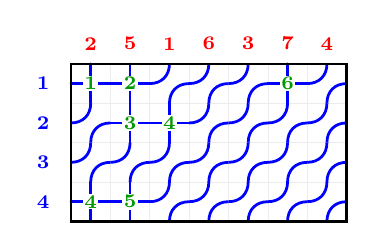
\begin{tikzpicture}[scale=0.5]
  \draw[lightgray, very thin, opacity=0.3] (0,1) grid[step=1] (7,5);
  % Row 1: crossings at 1,2,6
  \draw[blue, line width=1.0pt, line cap=round] (0,4.5) -- (1,4.5);
  \draw[blue, line width=1.0pt, line cap=round] (0.5,4) -- (0.5,5);
  \draw[blue, line width=1.0pt, line cap=round] (1,4.5) -- (2,4.5);
  \draw[blue, line width=1.0pt, line cap=round] (1.5,4) -- (1.5,5);
  \draw[blue, line width=1.0pt] (2,4.5) .. controls (2.3,4.5) and (2.5,4.7) .. (2.5,5);
  \draw[blue, line width=1.0pt] (2.5,4) .. controls (2.5,4.3) and (2.7,4.5) .. (3,4.5);
  \draw[blue, line width=1.0pt] (3,4.5) .. controls (3.3,4.5) and (3.5,4.7) .. (3.5,5);
  \draw[blue, line width=1.0pt] (3.5,4) .. controls (3.5,4.3) and (3.7,4.5) .. (4,4.5);
  \draw[blue, line width=1.0pt] (4,4.5) .. controls (4.3,4.5) and (4.5,4.7) .. (4.5,5);
  \draw[blue, line width=1.0pt] (4.5,4) .. controls (4.5,4.3) and (4.7,4.5) .. (5,4.5);
  \draw[blue, line width=1.0pt, line cap=round] (5,4.5) -- (6,4.5);
  \draw[blue, line width=1.0pt, line cap=round] (5.5,4) -- (5.5,5);
  \draw[blue, line width=1.0pt] (6,4.5) .. controls (6.3,4.5) and (6.5,4.7) .. (6.5,5);
  \draw[blue, line width=1.0pt] (6.5,4) .. controls (6.5,4.3) and (6.7,4.5) .. (7,4.5);
  % Row 2: crossings at 2,3
  \draw[blue, line width=1.0pt] (0,3.5) .. controls (0.3,3.5) and (0.5,3.7) .. (0.5,4);
  \draw[blue, line width=1.0pt] (0.5,3) .. controls (0.5,3.3) and (0.7,3.5) .. (1,3.5);
  \draw[blue, line width=1.0pt, line cap=round] (1,3.5) -- (2,3.5);
  \draw[blue, line width=1.0pt, line cap=round] (1.5,3) -- (1.5,4);
  \draw[blue, line width=1.0pt, line cap=round] (2,3.5) -- (3,3.5);
  \draw[blue, line width=1.0pt, line cap=round] (2.5,3) -- (2.5,4);
  \draw[blue, line width=1.0pt] (3,3.5) .. controls (3.3,3.5) and (3.5,3.7) .. (3.5,4);
  \draw[blue, line width=1.0pt] (3.5,3) .. controls (3.5,3.3) and (3.7,3.5) .. (4,3.5);
  \draw[blue, line width=1.0pt] (4,3.5) .. controls (4.3,3.5) and (4.5,3.7) .. (4.5,4);
  \draw[blue, line width=1.0pt] (4.5,3) .. controls (4.5,3.3) and (4.7,3.5) .. (5,3.5);
  \draw[blue, line width=1.0pt] (5,3.5) .. controls (5.3,3.5) and (5.5,3.7) .. (5.5,4);
  \draw[blue, line width=1.0pt] (5.5,3) .. controls (5.5,3.3) and (5.7,3.5) .. (6,3.5);
  \draw[blue, line width=1.0pt] (6,3.5) .. controls (6.3,3.5) and (6.5,3.7) .. (6.5,4);
  \draw[blue, line width=1.0pt] (6.5,3) .. controls (6.5,3.3) and (6.7,3.5) .. (7,3.5);
  % Row 3: empty
  \draw[blue, line width=1.0pt] (0,2.5) .. controls (0.3,2.5) and (0.5,2.7) .. (0.5,3);
  \draw[blue, line width=1.0pt] (0.5,2) .. controls (0.5,2.3) and (0.7,2.5) .. (1,2.5);
  \draw[blue, line width=1.0pt] (1,2.5) .. controls (1.3,2.5) and (1.5,2.7) .. (1.5,3);
  \draw[blue, line width=1.0pt] (1.5,2) .. controls (1.5,2.3) and (1.7,2.5) .. (2,2.5);
  \draw[blue, line width=1.0pt] (2,2.5) .. controls (2.3,2.5) and (2.5,2.7) .. (2.5,3);
  \draw[blue, line width=1.0pt] (2.5,2) .. controls (2.5,2.3) and (2.7,2.5) .. (3,2.5);
  \draw[blue, line width=1.0pt] (3,2.5) .. controls (3.3,2.5) and (3.5,2.7) .. (3.5,3);
  \draw[blue, line width=1.0pt] (3.5,2) .. controls (3.5,2.3) and (3.7,2.5) .. (4,2.5);
  \draw[blue, line width=1.0pt] (4,2.5) .. controls (4.3,2.5) and (4.5,2.7) .. (4.5,3);
  \draw[blue, line width=1.0pt] (4.5,2) .. controls (4.5,2.3) and (4.7,2.5) .. (5,2.5);
  \draw[blue, line width=1.0pt] (5,2.5) .. controls (5.3,2.5) and (5.5,2.7) .. (5.5,3);
  \draw[blue, line width=1.0pt] (5.5,2) .. controls (5.5,2.3) and (5.7,2.5) .. (6,2.5);
  \draw[blue, line width=1.0pt] (6,2.5) .. controls (6.3,2.5) and (6.5,2.7) .. (6.5,3);
  \draw[blue, line width=1.0pt] (6.5,2) .. controls (6.5,2.3) and (6.7,2.5) .. (7,2.5);
  % Row 4: crossings at 1,2
  \draw[blue, line width=1.0pt, line cap=round] (0,1.5) -- (1,1.5);
  \draw[blue, line width=1.0pt, line cap=round] (0.5,1) -- (0.5,2);
  \draw[blue, line width=1.0pt, line cap=round] (1,1.5) -- (2,1.5);
  \draw[blue, line width=1.0pt, line cap=round] (1.5,1) -- (1.5,2);
  \draw[blue, line width=1.0pt] (2,1.5) .. controls (2.3,1.5) and (2.5,1.7) .. (2.5,2);
  \draw[blue, line width=1.0pt] (2.5,1) .. controls (2.5,1.3) and (2.7,1.5) .. (3,1.5);
  \draw[blue, line width=1.0pt] (3,1.5) .. controls (3.3,1.5) and (3.5,1.7) .. (3.5,2);
  \draw[blue, line width=1.0pt] (3.5,1) .. controls (3.5,1.3) and (3.7,1.5) .. (4,1.5);
  \draw[blue, line width=1.0pt] (4,1.5) .. controls (4.3,1.5) and (4.5,1.7) .. (4.5,2);
  \draw[blue, line width=1.0pt] (4.5,1) .. controls (4.5,1.3) and (4.7,1.5) .. (5,1.5);
  \draw[blue, line width=1.0pt] (5,1.5) .. controls (5.3,1.5) and (5.5,1.7) .. (5.5,2);
  \draw[blue, line width=1.0pt] (5.5,1) .. controls (5.5,1.3) and (5.7,1.5) .. (6,1.5);
  \draw[blue, line width=1.0pt] (6,1.5) .. controls (6.3,1.5) and (6.5,1.7) .. (6.5,2);
  \draw[blue, line width=1.0pt] (6.5,1) .. controls (6.5,1.3) and (6.7,1.5) .. (7,1.5);
  \node[font=\scriptsize\bfseries, text=green!60!black, fill=white, inner sep=0.5pt] at (0.5,4.5) {1};
  \node[font=\scriptsize\bfseries, text=green!60!black, fill=white, inner sep=0.5pt] at (1.5,4.5) {2};
  \node[font=\scriptsize\bfseries, text=green!60!black, fill=white, inner sep=0.5pt] at (5.5,4.5) {6};
  \node[font=\scriptsize\bfseries, text=green!60!black, fill=white, inner sep=0.5pt] at (1.5,3.5) {3};
  \node[font=\scriptsize\bfseries, text=green!60!black, fill=white, inner sep=0.5pt] at (2.5,3.5) {4};
  \node[font=\scriptsize\bfseries, text=green!60!black, fill=white, inner sep=0.5pt] at (0.5,1.5) {4};
  \node[font=\scriptsize\bfseries, text=green!60!black, fill=white, inner sep=0.5pt] at (1.5,1.5) {5};
  \node[font=\scriptsize\bfseries, text=blue, anchor=east] at (-0.3,4.5) {1};
  \node[font=\scriptsize\bfseries, text=blue, anchor=east] at (-0.3,3.5) {2};
  \node[font=\scriptsize\bfseries, text=blue, anchor=east] at (-0.3,2.5) {3};
  \node[font=\scriptsize\bfseries, text=blue, anchor=east] at (-0.3,1.5) {4};
  % Output permutation at top
  \node[font=\scriptsize\bfseries, text=red, anchor=south] at (0.5,5.1) {2};
  \node[font=\scriptsize\bfseries, text=red, anchor=south] at (1.5,5.1) {5};
  \node[font=\scriptsize\bfseries, text=red, anchor=south] at (2.5,5.1) {1};
  \node[font=\scriptsize\bfseries, text=red, anchor=south] at (3.5,5.1) {6};
  \node[font=\scriptsize\bfseries, text=red, anchor=south] at (4.5,5.1) {3};
  \node[font=\scriptsize\bfseries, text=red, anchor=south] at (5.5,5.1) {7};
  \node[font=\scriptsize\bfseries, text=red, anchor=south] at (6.5,5.1) {4};
  \draw[black, line width=1.0pt] (0,1) rectangle (7,5);
\end{tikzpicture}
\caption*{(a) $R$ with $p=3$}
\end{minipage}
\hfill
% Step 2: After deletion
\begin{minipage}{0.22\textwidth}
\centering
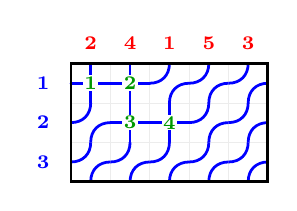
\begin{tikzpicture}[scale=0.5]
  \draw[lightgray, very thin, opacity=0.3] (0,2) grid[step=1] (5,5);
  % Row 1: crossings at 1,2 (no 6)
  \draw[blue, line width=1.0pt, line cap=round] (0,4.5) -- (1,4.5);
  \draw[blue, line width=1.0pt, line cap=round] (0.5,4) -- (0.5,5);
  \draw[blue, line width=1.0pt, line cap=round] (1,4.5) -- (2,4.5);
  \draw[blue, line width=1.0pt, line cap=round] (1.5,4) -- (1.5,5);
  \draw[blue, line width=1.0pt] (2,4.5) .. controls (2.3,4.5) and (2.5,4.7) .. (2.5,5);
  \draw[blue, line width=1.0pt] (2.5,4) .. controls (2.5,4.3) and (2.7,4.5) .. (3,4.5);
  \draw[blue, line width=1.0pt] (3,4.5) .. controls (3.3,4.5) and (3.5,4.7) .. (3.5,5);
  \draw[blue, line width=1.0pt] (3.5,4) .. controls (3.5,4.3) and (3.7,4.5) .. (4,4.5);
  \draw[blue, line width=1.0pt] (4,4.5) .. controls (4.3,4.5) and (4.5,4.7) .. (4.5,5);
  \draw[blue, line width=1.0pt] (4.5,4) .. controls (4.5,4.3) and (4.7,4.5) .. (5,4.5);
  % Row 2: crossings at 2,3
  \draw[blue, line width=1.0pt] (0,3.5) .. controls (0.3,3.5) and (0.5,3.7) .. (0.5,4);
  \draw[blue, line width=1.0pt] (0.5,3) .. controls (0.5,3.3) and (0.7,3.5) .. (1,3.5);
  \draw[blue, line width=1.0pt, line cap=round] (1,3.5) -- (2,3.5);
  \draw[blue, line width=1.0pt, line cap=round] (1.5,3) -- (1.5,4);
  \draw[blue, line width=1.0pt, line cap=round] (2,3.5) -- (3,3.5);
  \draw[blue, line width=1.0pt, line cap=round] (2.5,3) -- (2.5,4);
  \draw[blue, line width=1.0pt] (3,3.5) .. controls (3.3,3.5) and (3.5,3.7) .. (3.5,4);
  \draw[blue, line width=1.0pt] (3.5,3) .. controls (3.5,3.3) and (3.7,3.5) .. (4,3.5);
  \draw[blue, line width=1.0pt] (4,3.5) .. controls (4.3,3.5) and (4.5,3.7) .. (4.5,4);
  \draw[blue, line width=1.0pt] (4.5,3) .. controls (4.5,3.3) and (4.7,3.5) .. (5,3.5);
  % Row 3: empty
  \draw[blue, line width=1.0pt] (0,2.5) .. controls (0.3,2.5) and (0.5,2.7) .. (0.5,3);
  \draw[blue, line width=1.0pt] (0.5,2) .. controls (0.5,2.3) and (0.7,2.5) .. (1,2.5);
  \draw[blue, line width=1.0pt] (1,2.5) .. controls (1.3,2.5) and (1.5,2.7) .. (1.5,3);
  \draw[blue, line width=1.0pt] (1.5,2) .. controls (1.5,2.3) and (1.7,2.5) .. (2,2.5);
  \draw[blue, line width=1.0pt] (2,2.5) .. controls (2.3,2.5) and (2.5,2.7) .. (2.5,3);
  \draw[blue, line width=1.0pt] (2.5,2) .. controls (2.5,2.3) and (2.7,2.5) .. (3,2.5);
  \draw[blue, line width=1.0pt] (3,2.5) .. controls (3.3,2.5) and (3.5,2.7) .. (3.5,3);
  \draw[blue, line width=1.0pt] (3.5,2) .. controls (3.5,2.3) and (3.7,2.5) .. (4,2.5);
  \draw[blue, line width=1.0pt] (4,2.5) .. controls (4.3,2.5) and (4.5,2.7) .. (4.5,3);
  \draw[blue, line width=1.0pt] (4.5,2) .. controls (4.5,2.3) and (4.7,2.5) .. (5,2.5);
  \node[font=\scriptsize\bfseries, text=green!60!black, fill=white, inner sep=0.5pt] at (0.5,4.5) {1};
  \node[font=\scriptsize\bfseries, text=green!60!black, fill=white, inner sep=0.5pt] at (1.5,4.5) {2};
  \node[font=\scriptsize\bfseries, text=green!60!black, fill=white, inner sep=0.5pt] at (1.5,3.5) {3};
  \node[font=\scriptsize\bfseries, text=green!60!black, fill=white, inner sep=0.5pt] at (2.5,3.5) {4};
  \node[font=\scriptsize\bfseries, text=blue, anchor=east] at (-0.3,4.5) {1};
  \node[font=\scriptsize\bfseries, text=blue, anchor=east] at (-0.3,3.5) {2};
  \node[font=\scriptsize\bfseries, text=blue, anchor=east] at (-0.3,2.5) {3};
  % Output permutation at top
  \node[font=\scriptsize\bfseries, text=red, anchor=south] at (0.5,5.1) {2};
  \node[font=\scriptsize\bfseries, text=red, anchor=south] at (1.5,5.1) {4};
  \node[font=\scriptsize\bfseries, text=red, anchor=south] at (2.5,5.1) {1};
  \node[font=\scriptsize\bfseries, text=red, anchor=south] at (3.5,5.1) {5};
  \node[font=\scriptsize\bfseries, text=red, anchor=south] at (4.5,5.1) {3};
  \draw[black, line width=1.0pt] (0,2) rectangle (5,5);
\end{tikzpicture}
\caption*{(b) After delete (1,6)}
\end{minipage}
\hfill
% Step 3: Zero out row 3
\begin{minipage}{0.22\textwidth}
\centering
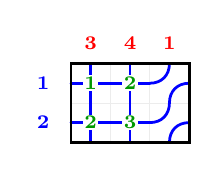
\begin{tikzpicture}[scale=0.5]
  \draw[lightgray, very thin, opacity=0.3] (0,3) grid[step=1] (3,5);
  % Row 1: crossings at 1,2
  \draw[blue, line width=1.0pt, line cap=round] (0,4.5) -- (1,4.5);
  \draw[blue, line width=1.0pt, line cap=round] (0.5,4) -- (0.5,5);
  \draw[blue, line width=1.0pt, line cap=round] (1,4.5) -- (2,4.5);
  \draw[blue, line width=1.0pt, line cap=round] (1.5,4) -- (1.5,5);
  \draw[blue, line width=1.0pt] (2,4.5) .. controls (2.3,4.5) and (2.5,4.7) .. (2.5,5);
  \draw[blue, line width=1.0pt] (2.5,4) .. controls (2.5,4.3) and (2.7,4.5) .. (3,4.5);
  % Row 2: crossings at 1,2
  \draw[blue, line width=1.0pt, line cap=round] (0,3.5) -- (1,3.5);
  \draw[blue, line width=1.0pt, line cap=round] (0.5,3) -- (0.5,4);
  \draw[blue, line width=1.0pt, line cap=round] (1,3.5) -- (2,3.5);
  \draw[blue, line width=1.0pt, line cap=round] (1.5,3) -- (1.5,4);
  \draw[blue, line width=1.0pt] (2,3.5) .. controls (2.3,3.5) and (2.5,3.7) .. (2.5,4);
  \draw[blue, line width=1.0pt] (2.5,3) .. controls (2.5,3.3) and (2.7,3.5) .. (3,3.5);
  \node[font=\scriptsize\bfseries, text=green!60!black, fill=white, inner sep=0.5pt] at (0.5,4.5) {1};
  \node[font=\scriptsize\bfseries, text=green!60!black, fill=white, inner sep=0.5pt] at (1.5,4.5) {2};
  \node[font=\scriptsize\bfseries, text=green!60!black, fill=white, inner sep=0.5pt] at (0.5,3.5) {2};
  \node[font=\scriptsize\bfseries, text=green!60!black, fill=white, inner sep=0.5pt] at (1.5,3.5) {3};
  \node[font=\scriptsize\bfseries, text=blue, anchor=east] at (-0.3,4.5) {1};
  \node[font=\scriptsize\bfseries, text=blue, anchor=east] at (-0.3,3.5) {2};
  % Output permutation at top
  \node[font=\scriptsize\bfseries, text=red, anchor=south] at (0.5,5.1) {3};
  \node[font=\scriptsize\bfseries, text=red, anchor=south] at (1.5,5.1) {4};
  \node[font=\scriptsize\bfseries, text=red, anchor=south] at (2.5,5.1) {1};
  \draw[black, line width=1.0pt] (0,3) rectangle (3,5);
\end{tikzpicture}
\caption*{(c) $\zeromap(\overline{R})$}
\end{minipage}
\hfill
% Step 4: Insert back
\begin{minipage}{0.22\textwidth}
\centering
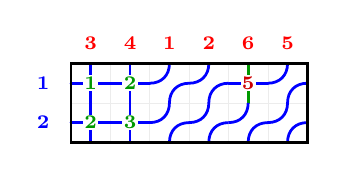
\begin{tikzpicture}[scale=0.5]
  \draw[lightgray, very thin, opacity=0.3] (0,3) grid[step=1] (6,5);
  % Row 1: crossings at 1,2,5
  \draw[blue, line width=1.0pt, line cap=round] (0,4.5) -- (1,4.5);
  \draw[blue, line width=1.0pt, line cap=round] (0.5,4) -- (0.5,5);
  \draw[blue, line width=1.0pt, line cap=round] (1,4.5) -- (2,4.5);
  \draw[blue, line width=1.0pt, line cap=round] (1.5,4) -- (1.5,5);
  \draw[blue, line width=1.0pt] (2,4.5) .. controls (2.3,4.5) and (2.5,4.7) .. (2.5,5);
  \draw[blue, line width=1.0pt] (2.5,4) .. controls (2.5,4.3) and (2.7,4.5) .. (3,4.5);
  \draw[blue, line width=1.0pt] (3,4.5) .. controls (3.3,4.5) and (3.5,4.7) .. (3.5,5);
  \draw[blue, line width=1.0pt] (3.5,4) .. controls (3.5,4.3) and (3.7,4.5) .. (4,4.5);
  \draw[blue, line width=1.0pt, line cap=round] (4,4.5) -- (5,4.5);
  \draw[green!60!black, line width=1.0pt, line cap=round] (4.5,4) -- (4.5,5);
  \draw[blue, line width=1.0pt] (5,4.5) .. controls (5.3,4.5) and (5.5,4.7) .. (5.5,5);
  \draw[blue, line width=1.0pt] (5.5,4) .. controls (5.5,4.3) and (5.7,4.5) .. (6,4.5);
  % Row 2: crossings at 1,2
  \draw[blue, line width=1.0pt, line cap=round] (0,3.5) -- (1,3.5);
  \draw[blue, line width=1.0pt, line cap=round] (0.5,3) -- (0.5,4);
  \draw[blue, line width=1.0pt, line cap=round] (1,3.5) -- (2,3.5);
  \draw[blue, line width=1.0pt, line cap=round] (1.5,3) -- (1.5,4);
  \draw[blue, line width=1.0pt] (2,3.5) .. controls (2.3,3.5) and (2.5,3.7) .. (2.5,4);
  \draw[blue, line width=1.0pt] (2.5,3) .. controls (2.5,3.3) and (2.7,3.5) .. (3,3.5);
  \draw[blue, line width=1.0pt] (3,3.5) .. controls (3.3,3.5) and (3.5,3.7) .. (3.5,4);
  \draw[blue, line width=1.0pt] (3.5,3) .. controls (3.5,3.3) and (3.7,3.5) .. (4,3.5);
  \draw[blue, line width=1.0pt] (4,3.5) .. controls (4.3,3.5) and (4.5,3.7) .. (4.5,4);
  \draw[blue, line width=1.0pt] (4.5,3) .. controls (4.5,3.3) and (4.7,3.5) .. (5,3.5);
  \draw[blue, line width=1.0pt] (5,3.5) .. controls (5.3,3.5) and (5.5,3.7) .. (5.5,4);
  \draw[blue, line width=1.0pt] (5.5,3) .. controls (5.5,3.3) and (5.7,3.5) .. (6,3.5);
  \node[font=\scriptsize\bfseries, text=green!60!black, fill=white, inner sep=0.5pt] at (0.5,4.5) {1};
  \node[font=\scriptsize\bfseries, text=green!60!black, fill=white, inner sep=0.5pt] at (1.5,4.5) {2};
  \node[font=\scriptsize\bfseries, text=red!80!black, fill=white, inner sep=0.5pt] at (4.5,4.5) {5};
  \node[font=\scriptsize\bfseries, text=green!60!black, fill=white, inner sep=0.5pt] at (0.5,3.5) {2};
  \node[font=\scriptsize\bfseries, text=green!60!black, fill=white, inner sep=0.5pt] at (1.5,3.5) {3};
  \node[font=\scriptsize\bfseries, text=blue, anchor=east] at (-0.3,4.5) {1};
  \node[font=\scriptsize\bfseries, text=blue, anchor=east] at (-0.3,3.5) {2};
  % Output permutation at top
  \node[font=\scriptsize\bfseries, text=red, anchor=south] at (0.5,5.1) {3};
  \node[font=\scriptsize\bfseries, text=red, anchor=south] at (1.5,5.1) {4};
  \node[font=\scriptsize\bfseries, text=red, anchor=south] at (2.5,5.1) {1};
  \node[font=\scriptsize\bfseries, text=red, anchor=south] at (3.5,5.1) {2};
  \node[font=\scriptsize\bfseries, text=red, anchor=south] at (4.5,5.1) {6};
  \node[font=\scriptsize\bfseries, text=red, anchor=south] at (5.5,5.1) {5};
  \draw[black, line width=1.0pt] (0,3) rectangle (6,5);
\end{tikzpicture}
\caption*{(d) After $\ins{5}{1}$}
\end{minipage}

\vspace{0.3cm}

% Step 5: Final with R>p
\begin{minipage}{0.45\textwidth}
\centering
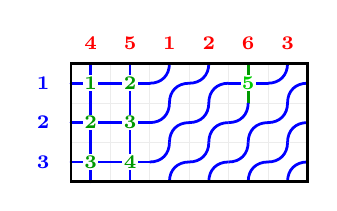
\begin{tikzpicture}[scale=0.5]
  \draw[lightgray, very thin, opacity=0.3] (0,1) grid[step=1] (6,4);
  % Row 1: crossings at 1,2,5
  \draw[blue, line width=1.0pt, line cap=round] (0,3.5) -- (1,3.5);
  \draw[blue, line width=1.0pt, line cap=round] (0.5,3) -- (0.5,4);
  \draw[blue, line width=1.0pt, line cap=round] (1,3.5) -- (2,3.5);
  \draw[blue, line width=1.0pt, line cap=round] (1.5,3) -- (1.5,4);
  \draw[blue, line width=1.0pt] (2,3.5) .. controls (2.3,3.5) and (2.5,3.7) .. (2.5,4);
  \draw[blue, line width=1.0pt] (2.5,3) .. controls (2.5,3.3) and (2.7,3.5) .. (3,3.5);
  \draw[blue, line width=1.0pt] (3,3.5) .. controls (3.3,3.5) and (3.5,3.7) .. (3.5,4);
  \draw[blue, line width=1.0pt] (3.5,3) .. controls (3.5,3.3) and (3.7,3.5) .. (4,3.5);
  \draw[blue, line width=1.0pt, line cap=round] (4,3.5) -- (5,3.5);
  \draw[green!60!black, line width=1.0pt, line cap=round] (4.5,3) -- (4.5,4);
  \draw[blue, line width=1.0pt] (5,3.5) .. controls (5.3,3.5) and (5.5,3.7) .. (5.5,4);
  \draw[blue, line width=1.0pt] (5.5,3) .. controls (5.5,3.3) and (5.7,3.5) .. (6,3.5);
  % Row 2: crossings at 1,2
  \draw[blue, line width=1.0pt, line cap=round] (0,2.5) -- (1,2.5);
  \draw[blue, line width=1.0pt, line cap=round] (0.5,2) -- (0.5,3);
  \draw[blue, line width=1.0pt, line cap=round] (1,2.5) -- (2,2.5);
  \draw[blue, line width=1.0pt, line cap=round] (1.5,2) -- (1.5,3);
  \draw[blue, line width=1.0pt] (2,2.5) .. controls (2.3,2.5) and (2.5,2.7) .. (2.5,3);
  \draw[blue, line width=1.0pt] (2.5,2) .. controls (2.5,2.3) and (2.7,2.5) .. (3,2.5);
  \draw[blue, line width=1.0pt] (3,2.5) .. controls (3.3,2.5) and (3.5,2.7) .. (3.5,3);
  \draw[blue, line width=1.0pt] (3.5,2) .. controls (3.5,2.3) and (3.7,2.5) .. (4,2.5);
  \draw[blue, line width=1.0pt] (4,2.5) .. controls (4.3,2.5) and (4.5,2.7) .. (4.5,3);
  \draw[blue, line width=1.0pt] (4.5,2) .. controls (4.5,2.3) and (4.7,2.5) .. (5,2.5);
  \draw[blue, line width=1.0pt] (5,2.5) .. controls (5.3,2.5) and (5.5,2.7) .. (5.5,3);
  \draw[blue, line width=1.0pt] (5.5,2) .. controls (5.5,2.3) and (5.7,2.5) .. (6,2.5);
  % Row 3: crossings at 1,2 (from R>p shifted)
  \draw[blue, line width=1.0pt, line cap=round] (0,1.5) -- (1,1.5);
  \draw[blue, line width=1.0pt, line cap=round] (0.5,1) -- (0.5,2);
  \draw[blue, line width=1.0pt, line cap=round] (1,1.5) -- (2,1.5);
  \draw[blue, line width=1.0pt, line cap=round] (1.5,1) -- (1.5,2);
  \draw[blue, line width=1.0pt] (2,1.5) .. controls (2.3,1.5) and (2.5,1.7) .. (2.5,2);
  \draw[blue, line width=1.0pt] (2.5,1) .. controls (2.5,1.3) and (2.7,1.5) .. (3,1.5);
  \draw[blue, line width=1.0pt] (3,1.5) .. controls (3.3,1.5) and (3.5,1.7) .. (3.5,2);
  \draw[blue, line width=1.0pt] (3.5,1) .. controls (3.5,1.3) and (3.7,1.5) .. (4,1.5);
  \draw[blue, line width=1.0pt] (4,1.5) .. controls (4.3,1.5) and (4.5,1.7) .. (4.5,2);
  \draw[blue, line width=1.0pt] (4.5,1) .. controls (4.5,1.3) and (4.7,1.5) .. (5,1.5);
  \draw[blue, line width=1.0pt] (5,1.5) .. controls (5.3,1.5) and (5.5,1.7) .. (5.5,2);
  \draw[blue, line width=1.0pt] (5.5,1) .. controls (5.5,1.3) and (5.7,1.5) .. (6,1.5);
  \node[font=\scriptsize\bfseries, text=green!60!black, fill=white, inner sep=0.5pt] at (0.5,3.5) {1};
  \node[font=\scriptsize\bfseries, text=green!60!black, fill=white, inner sep=0.5pt] at (1.5,3.5) {2};
  \node[font=\scriptsize\bfseries, text=green!80!black, fill=white, inner sep=0.5pt] at (4.5,3.5) {5};
  \node[font=\scriptsize\bfseries, text=green!60!black, fill=white, inner sep=0.5pt] at (0.5,2.5) {2};
  \node[font=\scriptsize\bfseries, text=green!60!black, fill=white, inner sep=0.5pt] at (1.5,2.5) {3};
  \node[font=\scriptsize\bfseries, text=green!60!black, fill=white, inner sep=0.5pt] at (0.5,1.5) {3};
  \node[font=\scriptsize\bfseries, text=green!60!black, fill=white, inner sep=0.5pt] at (1.5,1.5) {4};
  \node[font=\scriptsize\bfseries, text=blue, anchor=east] at (-0.3,3.5) {1};
  \node[font=\scriptsize\bfseries, text=blue, anchor=east] at (-0.3,2.5) {2};
  \node[font=\scriptsize\bfseries, text=blue, anchor=east] at (-0.3,1.5) {3};
  % Output permutation at top
  \node[font=\scriptsize\bfseries, text=red, anchor=south] at (0.5,4.1) {4};
  \node[font=\scriptsize\bfseries, text=red, anchor=south] at (1.5,4.1) {5};
  \node[font=\scriptsize\bfseries, text=red, anchor=south] at (2.5,4.1) {1};
  \node[font=\scriptsize\bfseries, text=red, anchor=south] at (3.5,4.1) {2};
  \node[font=\scriptsize\bfseries, text=red, anchor=south] at (4.5,4.1) {6};
  \node[font=\scriptsize\bfseries, text=red, anchor=south] at (5.5,4.1) {3};
  \draw[black, line width=1.0pt] (0,1) rectangle (6,4);
\end{tikzpicture}
\caption*{(e) Final $\qr_p(R)$ with $R_{>p}$ reattached}
\end{minipage}

\caption{Example of $\qr_p$ operation with $p=3$. Starting with (a) $R$ where row 3 is empty, we identify element $(1,6)$ creates maxd $> p$. (b) After deleting it (storing row 1 in $A_1$). (c) Apply $\zeromap$ to get 2-row graph. (d) Insert back at row 1 with $k=d_1-1=5$ (shown in red). (e) Reattach $R_{>p}$ shifted down to get final result.}
\label{figure:zpexample}
\end{figure}

\begin{definition}
Let $R$ be an RC graph. We define an RC graph $\overline{R}$ and a sequence $\mathtt{strip}(R)$ as follows. Let $\maxd(R)=n$, set $R_0=R$, and set $A_0=()$. While $\maxd(R_i)> n -1$, delete the element $(a,b)\in R_i$ such that $\rtt_{R_i}(a,b)=(\maxd(R_i), \maxd(R_i) + 1)$ to obtain $R_{i+1}$, and add $a$ to $A_i$ to obtain $A_{i+1}$. When the algorithm terminates at step $k$, set
$$\mathtt{strip}(R) = A_k$$
and set $\overline{R} = \overline{R}$.
\end{definition}

\begin{lemma} \label{lemma:reconstruct}
Let $R$ be an RC graph. Then
$$R = \ins{\maxd(R)}{\mathtt{strip}(R)} \overline{R}$$
\end{lemma}
\begin{proof}
Let $n=\maxd(R)$. We prove this by induction on $\code_n(R)$. Let $(i,j)$ be the location of the descent $n$ in $R$. If $\code_n(R)=1$, then we know that insertion of $i$ into $\overline{R}$ returns an RC graph with the same weight and permutation as $R$, the latter assertion because the only $n$-reflection that increases the length of $\wof{\overline{R}}$ by exactly $1$ is $s_n$. By the exchange property, there is precisely one location in row $i$ that this $n$-reflection can be inserted, and we have the result when $\code_{n}(R)=1$.

Assume the inductive hypothesis that we have the result for $\code_n(R) = k$ for some $k\geq 1$ and additionally that insertion order of reflections has been $(n, n+1),\ldots,(n,n+k)$. Assume $\mathtt{strip}(R) = (r_1,\ldots,r_{k+1})$ in increasing order and we have inserted all of $r_2,\ldots,r_{k+1}$ in Algorithm \ref{algorithm:insertion}. By the induction hypothesis, the RC graph $R'$ we have at this point has permutation $\code_i{R'} = \code_i{R}$ for $i<n$ and $\code_n(R') = k$, and we have equality of $R'$ with $R$ except deletion of the root $(n, n+k + 1)$. Since $\wof{R'}(n) < \wof{R'}(n+k+1)$, the only $n$-reflection that can be inserted to increase the length of $\wof{R'}$ by $1$ is $(n, n+k+1)$. By pipe considerations, this must be inserted in column $c = n + k + 1 - r_1$. Since this is the only possible insertion location and the permutation is the same as $\wof{R}$, we have the result by induction.
\end{proof}


\begin{theorem}
Let $R\in\BRC(w,n)^{(0,p)}$ be the set of all bounded RC graphs with $\hr(R)=n$ such that row $p$ of $R$ is empty. Then we have that the restriction of $\qr_p$ is a bijection
$$\qr_p:\BRC(w,n)^{(0,p)}\to\bigcup_{\substack{w\downvar{p} w'\\\ell(w)=\ell(w')}} \BRC(w', n-1)$$
satisfying $\wtt(\qr_p(R)) = (i_1,\ldots,i_{p-1},i_{p+1},\ldots,i_{n})$, where $\wtt(R)=(i_1,\ldots,i_n)$.
\end{theorem}
\begin{proof}
Consider first the special case that $R_{>p}$ is empty. Let $w_0 = \wof{\zeromap(\overline{R})}$. Then we know that
$$\overline{R}\downvar{p} \zeromap(\overline{R})$$
Since every element of $A_k$ is less than $p$ and $d_k>p$, the insertion $\ins{d_k-1}{A_k}\zeromap(\overline{R})$ only adds right roots $(a,b)$ with $a<p$ and $b>p$. Thus
$$\ins{d_k}{A_k}\overline{R}\downvar{p} \ins{d_k-1}{A_k}\zeromap(\overline{R})$$
We assert the (descending) inductive hypothesis that for some index $j$ we have
$$\ins{d_j}{A_j}\cdots\ins{d_k}{A_k}\overline{R}\downvar{p} \ins{d_j-1}{A_j}\cdots\ins{d_k-1}{A_k}\zeromap(\overline{R})$$
Then the induction step follows with precisely the same reasoning; since every element of $A_{j-1}$ is less than $p$ and $d_{j-1}>p$, the insertion $\ins{d_{j-1}-1}{A_{j-1}}$ only adds right roots $(a,b)$ with $a<p$ and $b>p$. Thus
$$\ins{d_{j-1}}{A_{j-1}}\cdots\ins{d_k}{A_k}\overline{R}\downvar{p} \ins{d_{j-1}-1}{A_{j-1}}\cdots\ins{d_k-1}{A_k}\zeromap(\overline{R})$$
and the result follows by induction in the special case that $R_{>p}$ is empty, where we invoke Lemma \ref{lemma:reconstruct} to assert that the left-hand side is equal to $R$.

Since the row was initially empty, we have at our disposal the exchange property on $R_{>p}$, shifting the reflections down a row to obtain the general case.
\end{proof}

\begin{definition}
Define 
$$\ttrim_i = \qr_i\rcdd^i$$
\end{definition}

\cite{samuelmolev}
\bibliographystyle{acm}
\bibliography{schubert_bialgebra}


\end{document}
